\documentclass[11pt,a4paper]{article}
\usepackage{graphicx}
\usepackage{theorem}
\usepackage{color}
\usepackage{listings}

\title{MetaOS Architecture.}
\author{Sergio Alvarez (setelena@gmail.com),
    Luis F. Canals (luisf.canals@gmail.com)}

\begin{document}

\date{\today}
\maketitle


\section{Abstract}

\section{MetaOS modules.}

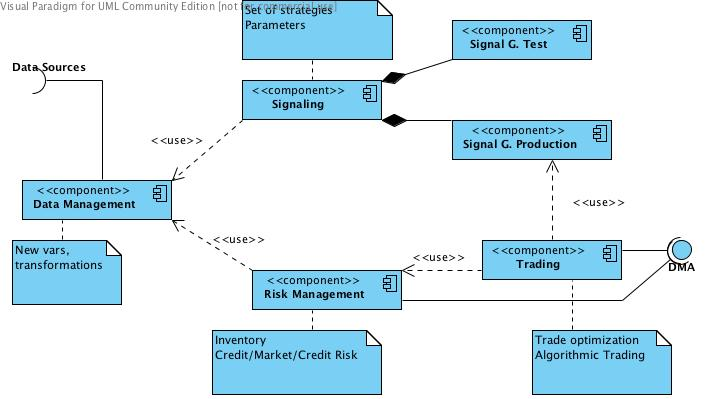
\includegraphics{images/Overview.jpg}

\section{Java packages.}
Quite similar information is available in Javadoc, maybe with more 
examples oriented to programming tasks.

In this section, we're trying to provide an architectural view 
and the ways system may grow.


\subsection{datamgt}
Classes related to data access, transformation and making of new variables.
Remote (on demand and on line trading systems) and even local datasources 
(like CSV files) are represented using a common interface thanks to 
this package.

Listener and factory patterns are in the core of the package to let:
    a.- the startegies work into a simulated environment (for instance
        created with historical data) and real time world agnostically,
        thus without changing anything into strategies code;

    b.- synthesize new data (in real time and in simulations) in an homogeneus
        way, providing the same appear for crude and synthesized data;

General package overview is shown is this figure, in which only interfaces
are represented. The other elements in package are classes implementing
interfaces for general cases (CSV files, sources with one or several symbols,
file splitting manipulation, etc)

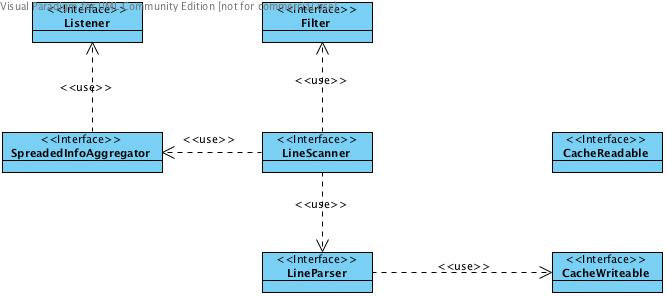
\includegraphics{images/datamgrClassDiagram.jpg}

The usage of the classes from this package is like this figure
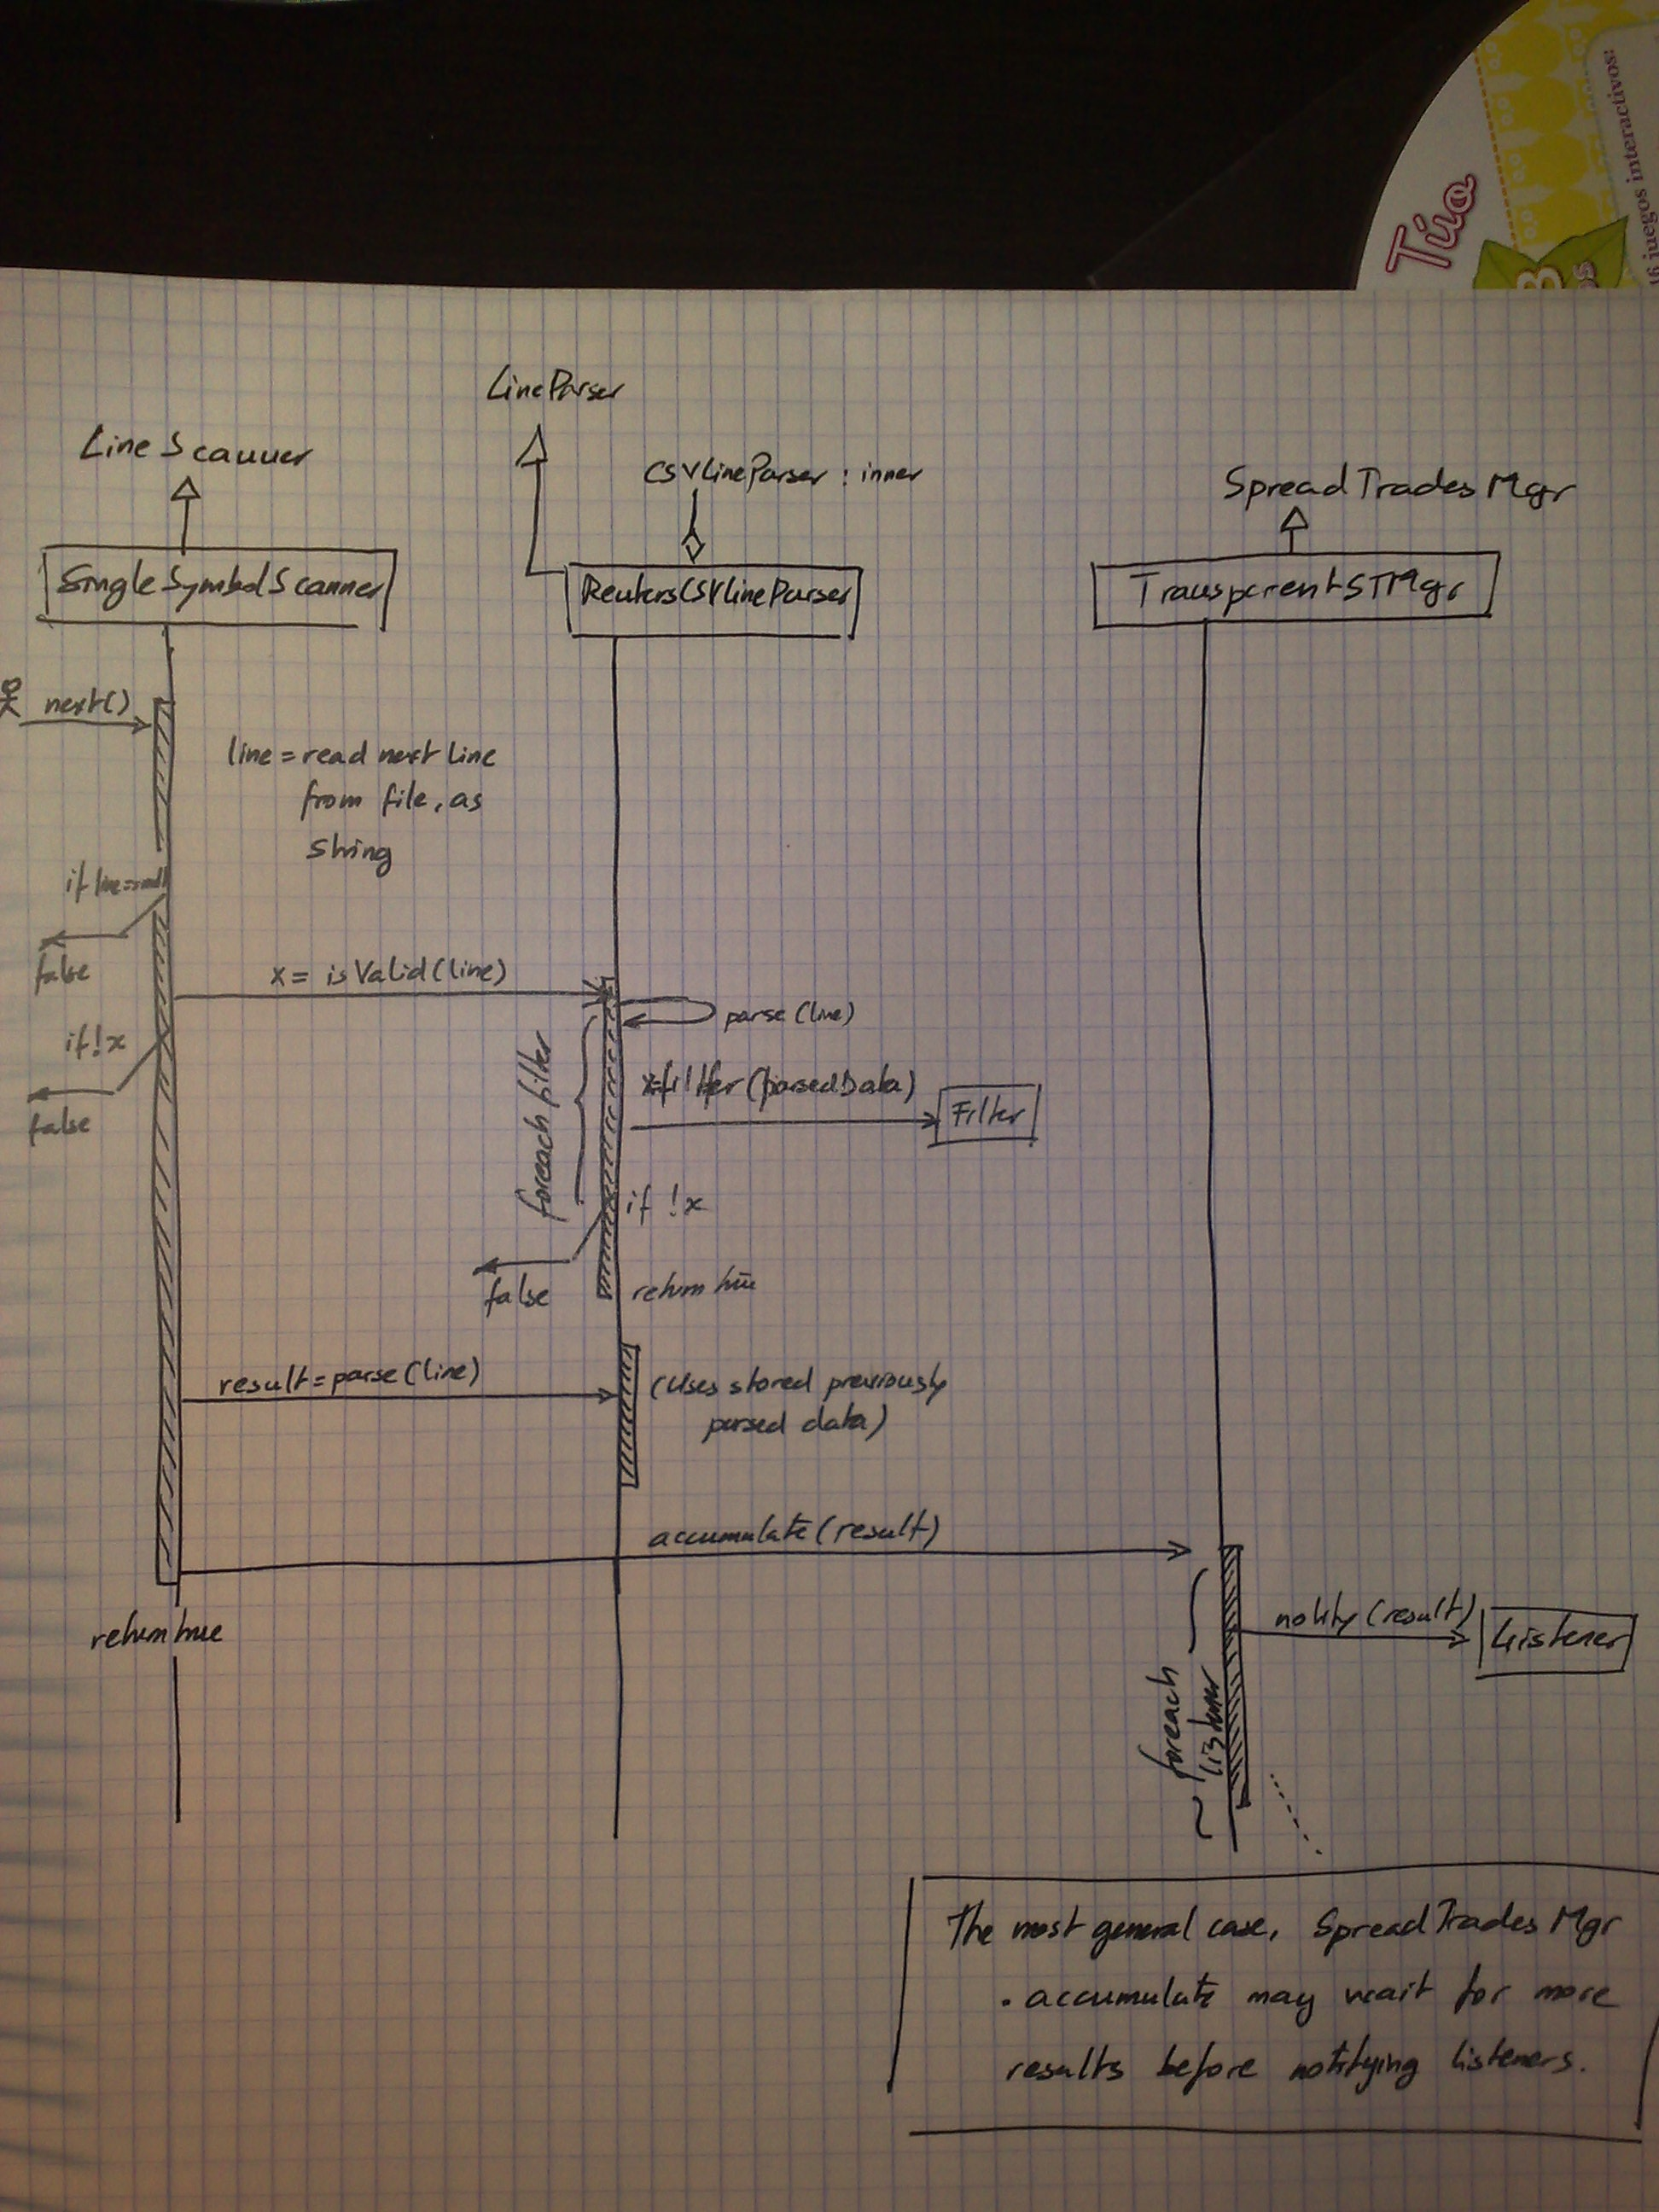
\includegraphics{images/datamgrsequence.jpg}

The only main principle driving the package is the concept of listener:
trading data is gotten from sources and several listeners are subscribed to
the data management classes; listeners are, for instance, predictors,
strategies or data transformations.

\subsection{engine}

\subsection{riskmgt}

\subsection{signalgrt}

\subsection{trading}

\subsection{util}

\subsection{ext}

\section{Integration with other languages}

\subsection{R project}

\subsection{Python}

\subsection{Any other}

\section{Examples --------- erase me, please}
Lorem ipsum dolor.

\lstset{language=Python,frame=single,tabsize=2,basicstyle=\tiny}
\lstinputlisting{../src/test/jython/testR.py}

As it's seen from the code, a R source code named \emph{correlation.r}
where a class \emph{correlator} is defined. The class should have got the
methods \emph{memo} and \emph{show}, as in this example:

\lstset{language=R,frame=single,tabsize=2,basicstyle=\tiny}
\lstinputlisting{../src/main/R/correlation.r}



\section{Generalization}

The following code (\emph{rintegration.py}) uses the same described principle 
in the previous section but letting the name of R source containing the 
class as a runtime parameter:

\lstset{language=Python,frame=single,tabsize=2,basicstyle=\tiny}
\lstinputlisting{../src/python/rintegration.py}

In this case, interface for R class has been modified, to create a simple
predictor with two methods, \emph{learn} and \emph{predict}. An example of
predictor based on linear regression might look like this:

From the example, we write down the interface all R-class should satisfy
to be compatible with \emph{rintegration.py} requirements (in pseudocode 
Java-like):

\lstset{language=Java,frame=single,tabsize=4,basicstyle=\tiny}
\begin{lstlisting}

    interface PredictorInR {
        // Learns a new relation x->y
        void learn(double x, double y);

        // Tries to predict the value of y from x
        double predict(double x);
    }

\end{lstlisting}
\label{PredictorInR}



\section{Usage from command line and visual interface}

The code in \emph{rintegration.py} can be invoked even from command line or
from visual interface. In both cases, file acting as a source of prices,
the main Python script (\emph{rintegration.py} in this case) and the R file
containing the source code of the class with the predictor following the 
interface described in the interface \ref{PredictorInR}.


\section{License terms}

This is a GNU Licensed Document. Modifications and copies of this document
must follow the GNU License, refering to authors and to the original document.
All other rights are reserved by the authors.
\end{document}
